\chapter{Foundations for Inference}
\label{FoundationForInference}

% Chapter intro
\begin{example}{Suppose your professor splits the students in class into two groups: students on the left and students on the right. If $\hat{p}_{_L}$ and $\hat{p}_{_R}$ represent the proportion of students who own an Apple product on the left and right, respectively, would you be surprised if $\hat{p}_{_L}$ did not {exactly} equal $\hat{p}_{_R}$?}\label{classRightLeftSideApple}
While the proportions would probably be close to each other, they are probably not exactly the same. We would probably observe a small difference due to {chance}.
\end{example}

\begin{exercise}
If we don't think the side of the room a person sits on in class is related to whether the person owns an Apple product, what assumption are we making about the relationship between these two variables?\footnote{We would be assuming that these two variables are \emph{independent}, meaning they are unrelated.}
\end{exercise}

Studying randomness of this form is a key focus of statistics. In~this chapter, we'll explore this type of randomness in the context of several applications, and we'll learn new tools and ideas that will be applied throughout the rest of the book.

%%%%
\section{Understanding inference through simulation}

%%? new section ?

%%%%
%_________________
\section{Randomization case study: gender discrimination}
\label{caseStudyGenderDiscrimination}

\index{data!discrimination|(}

We consider a study investigating gender discrimination in the 1970s, which is set in the context of personnel decisions within a bank.\footnote{Rosen B and Jerdee T. 1974. ``Influence of sex role stereotypes on personnel decisions.'' Journal of Applied Psychology 59(1):9-14.} The research question we hope to answer~is, ``Are females discriminated against in promotion decisions made by male managers?''

\subsection{Variability within data}
\label{variabilityWithinData}

The participants in this study were 48 male bank supervisors attending a management institute at the University of North Carolina in 1972. They were asked to assume the role of the personnel director of a bank and were given a personnel file to judge whether the person should be promoted to a branch manager position. The files given to the participants were identical, except that half of them indicated the candidate was male and the other half indicated the candidate was female. These files were randomly assigned to the subjects.

\begin{exercise}
Is this an observational study or an experiment? How does the type of study impact what can be inferred from the results?\footnote{The study is an experiment, as subjects were randomly assigned a male file or a female file. Since this is an experiment, the results can be used to evaluate a causal relationship between gender of a candidate and the promotion decision.}
\end{exercise}

For each supervisor we recorded the gender associated with the assigned file and the promotion decision. Using the results of the study summarized in Table~\ref{discriminationResults}, we would like to evaluate if females are unfairly discriminated against in promotion decisions. In this study, a smaller proportion of females are promoted than males (0.583 versus 0.875), but it is unclear whether the difference provides \emph{convincing evidence} that females are unfairly discriminated against.

\begin{table}[ht]
\centering
\begin{tabular}{l l cc rr}
& & \multicolumn{2}{c}{\var{decision}} \\
  \cline{3-4}
		&			& 	{promoted} 	& {not promoted} & Total & \hspace{3mm}  \\ 
  \cline{2-5}
		&	{male} 			& 21    		& 3   & 24  	 \\ 
  \raisebox{1.5ex}[0pt]{\var{gender}}		&	{female} 	& 14    		& 10     & 24	 \\ 
  \cline{2-5}
  		&	Total		& 35	& 13	&  48 \\
  \cline{2-5}
\end{tabular}
\caption{Summary results for the gender discrimination study.}
\label{discriminationResults}
\end{table}

\begin{example}{Statisticians are sometimes called upon to evaluate the strength of evidence. When looking at the rates of promotion for males and females in this study, why might we be tempted to immediately conclude that females are being discriminated against?}\label{discriminationResultsWhatIsConvincingEvidence}
The large difference in promotion rates (58.3\% for females versus 87.5\% for males) suggest there might be discrimination against women in promotion decisions. However, we cannot yet be sure if the observed difference represents discrimination or is just from random chance. Generally there is a little bit of fluctuation in sample data, and we wouldn't expect the sample proportions to be \emph{exactly} equal, even if the truth was that the promotion decisions were independent of gender.
\end{example}

Example~\ref{discriminationResultsWhatIsConvincingEvidence} is a reminder that the observed outcomes in the sample may not perfectly reflect the true relationships between variables in the underlying population. Table~\ref{discriminationResults} shows there were 7 fewer promotions in the female group than in the male group, a difference in promotion rates of 29.2\% $\left( \frac{21}{24} - \frac{14}{24} = 0.292 \right)$. This observed difference is what we call a \term{point estimate} of the true effect. The point estimate of the difference is large, but the sample size for the study is small, making it unclear if this observed difference represents discrimination or whether it is simply due to chance. We label these two competing claims, $H_0$ and $H_A$:
\begin{itemize}
\setlength{\itemsep}{0mm}
\item[$H_0$:] \textbf{Null hypothesis.} The variables \var{gender} and \var{decision} are independent. They have no relationship, and the observed difference between the proportion of males and females who were promoted, 29.2\%, was due to chance.
\item[$H_A$:] \textbf{Alternative hypothesis.} The variables \var{gender} and \var{decision} are \emph{not} independent. The difference in promotion rates of 29.2\% was not due to chance, and equally qualified females are less likely to be promoted than males.
\end{itemize}

\begin{termBox}{\tBoxTitle{Hypothesis testing}
These hypotheses are part of what is called a \term{hypothesis test}. A hypothesis test is a statistical technique used to evaluate competing claims using data. Often times, the null hypothesis takes a stance of \emph{no difference} or \emph{no effect}. If the null hypothesis and the data notably disagree, then we will reject the null hypothesis in favor of the alternative hypothesis. \vspace{3mm}

Don't worry if you aren't a master of hypothesis testing at the end of this section. We'll discuss these ideas and details many times in this chapter.}
\end{termBox}

What would it mean if the null hypothesis, which says the variables \var{gender} and \var{decision} are unrelated, is true? It would mean each banker would decide whether to promote the candidate without regard to the gender indicated on the file. That~is, the difference in the promotion percentages would be due to the way the files were randomly divided to the bankers, and the randomization just happened to give rise to a relatively large difference of 29.2\%.

Consider the alternative hypothesis: bankers were influenced by which gender was listed on the personnel file. If this was true, and especially if this influence was substantial, we would expect to see some difference in the promotion rates of male and female candidates. If this gender bias was against females, we would expect a smaller fraction of promotion recommendations for female personnel files relative to the male files.

We will choose between these two competing claims by assessing if the data conflict so much with $H_0$ that the null hypothesis cannot be deemed reasonable. If this is the case, and the data support $H_A$, then we will reject the notion of independence and conclude that these data provide strong evidence of discrimination.

\subsection{Simulating the study}
\label{simulatingTheStudy}

Table~\ref{discriminationResults} shows that 35 bank supervisors recommended promotion and 13 did not. Now, suppose the bankers' decisions were independent of gender. Then, if we conducted the experiment again with a different random assignment of files, differences in promotion rates would be based only on random fluctuation. We can actually perform this \term{randomization}, which simulates what would have happened if the bankers' decisions had been independent of gender but we had distributed the files differently.\footnote{The test procedure we employ in this section is formally called a \term{permutation test}.}

In this \term{simulation}, we thoroughly shuffle 48 personnel files, 24 labeled \resp{male} and 24 labeled \resp{female}, and deal these files into two stacks. We will deal 35 files into the first stack, which will represent the 35 supervisors who recommended promotion. The second stack will have 13 files, and it will represent the 13 supervisors who recommended against promotion. Then, as we did with the original data, we tabulate the results and determine the fraction of \resp{male} and \resp{female} who were promoted.

Since the randomization of files in this simulation is independent of the promotion decisions, any difference in the two fractions is entirely due to chance. Table~\ref{discriminationRand1} show the results of such a simulation.

\begin{table}[ht]
\centering
\begin{tabular}{l l cc rr}
& & \multicolumn{2}{c}{\var{decision}} \\
  \cline{3-4}
		&			& 	{promoted} 	& {not promoted} & Total & \hspace{3mm}  \\ 
  \cline{2-5}
		&	male 					& 18    		& 6    & 24 	 \\ 
  \raisebox{1.5ex}[0pt]{\var{gender\_\hspace{0.3mm}simulated}}		&	female 	& 17    		& 7 & 24    	 \\ 
  \cline{2-5}
  & Total	& 35 & 13 & 48
\end{tabular}
\caption{Simulation results, where any difference in promotion rates between \resp{male} and \resp{female} is purely due to chance.}
\label{discriminationRand1}
\end{table}

\textPE{\pagebreak}

\begin{exercise} \label{sampleDifferenceInMaleAndFemaleDiscrimination}
What is the difference in promotion rates between the two simulated groups in Table~\ref{discriminationRand1}? How does this compare to the observed difference 29.2\% from the actual~study?\footnote{$18/24 - 17/24=0.042$ or about 4.2\% in favor of the men. This difference due to chance is much smaller than the difference observed in the actual groups.}
\end{exercise}

\subsection{Checking for independence}

We computed one possible difference under the null hypothesis in Guided Practice~\ref{sampleDifferenceInMaleAndFemaleDiscrimination}, which represents one difference due to chance. While in this first simulation, we physically dealt out files, it is much more efficient to perform this simulation using a computer. Repeating the simulation on a computer, we get another difference due to chance: -0.042. And another: 0.208. And so on until we repeat the simulation enough times that we have a good idea of what represents the \emph{distribution of differences from chance alone}. Figure~\ref{discRandDotPlot} shows a plot of the differences found from 100 simulations, where each dot represents a simulated difference between the proportions of male and female files recommended for promotion.

\begin{figure}[ht]
\centering
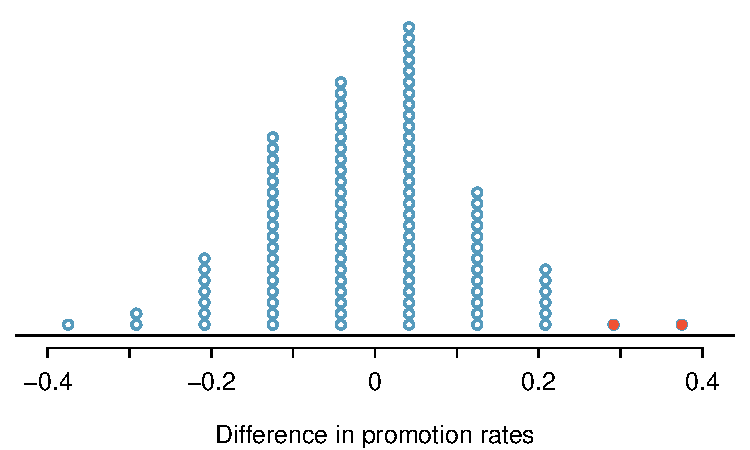
\includegraphics[width=0.65\textwidth]{05/figures/discRandDotPlot/discRandDotPlot}
\caption{A stacked dot plot of differences from 100 simulations produced under the null hypothesis, $H_0$, where \var{gender\_\hspace{0.3mm}simulated} and \var{decision} are independent. Two of the 100 simulations had a difference of at least 29.2\%, the difference observed in the study, and are shown as solid dots.}
\label{discRandDotPlot}
\end{figure}

Note that the distribution of these simulated differences is centered around 0. Because we simulated differences in a way that made no distinction between men and women, this makes sense: we should expect differences from chance alone to fall around zero with some random fluctuation for each simulation.

\begin{example}{How often would you observe a difference of at least 29.2\% (0.292) according to Figure~\ref{discRandDotPlot}? Often, sometimes, rarely, or never?}
It appears that a difference of at least 29.2\% due to chance alone would only happen about 2\% of the time according to Figure~\ref{discRandDotPlot}. Such a low probability indicates that observing such a large difference from chance is rare.
\end{example}

The difference of 29.2\% is a rare event if there really is no impact from listing gender in the candidates' files, which provides us with two possible interpretations of the study results:
\begin{itemize}
\setlength{\itemsep}{0mm}
\item[$H_0$:] \textbf{Null hypothesis.} Gender has no effect on promotion decision, and we observed a difference that is so large that it would only happen rarely.
\item[$H_A$:] \textbf{Alternative hypothesis.} Gender has an effect on promotion decision, and what we observed was actually due to equally qualified women being discriminated against in promotion decisions, which explains the large difference of 29.2\%.
\end{itemize}
When we conduct formal studies, we reject a skeptical position if the data strongly conflict with that position.%When we conduct formal studies, usually we reject the notion that we just happened to observe a rare event.
\footnote{This reasoning does not generally extend to anecdotal observations. Each of us observes incredibly rare events every day, events we could not possibly hope to predict. However, in the non-rigorous setting of anecdotal evidence, almost anything may appear to be a rare event, so the idea of looking for rare events in day-to-day activities is treacherous. For example, we might look at the lottery: there was only a 1 in 176 million chance that the Mega Millions numbers for the largest jackpot in history (March 30, 2012) would be (2, 4, 23, 38, 46) with a Mega ball of (23), but nonetheless those numbers came up! However, no matter what numbers had turned up, they would have had the same incredibly rare odds. That is, \emph{any set of numbers we could have observed would ultimately be incredibly rare}. This type of situation is typical of our daily lives: each possible event in itself seems incredibly rare, but if we consider every alternative, those outcomes are also incredibly rare. We should be cautious not to misinterpret such anecdotal evidence.} 
%In this case, we reject the null hypothesis in favor of the alternative. 
In our analysis, we determined that there was only a $\approx$2\% probability of obtaining a sample where $\geq$29.2\% more males than females get promoted by chance alone, so we conclude the data provide strong evidence of gender discrimination against women by the supervisors. In this case, we reject the null hypothesis in favor of the alternative.

\index{data!discrimination|)}

Statistical inference is the practice of making decisions and conclusions from data in the context of uncertainty. Errors do occur, just like rare events, and the data set at hand might lead us to the wrong conclusion. While a given data set may not always lead us to a correct conclusion, statistical inference gives us tools to control and evaluate how often these errors occur. Before getting into the nuances of hypothesis testing, let's work through another case study.


%%%%%
%_________________
\section{Randomization case study: opportunity cost}
\label{caseStudyOpportunityCost}

How rational and consistent is the behavior of the typical American college student? In~this section, we'll explore whether college student consumers always consider an obvious fact: money not spent now can be spent later.

In particular, we are interested in whether reminding students about this well-known fact about money causes them to be a little thriftier. A skeptic might think that such a reminder would have no impact. We can summarize these two perspectives using the null and alternative hypothesis framework.
\begin{itemize}
\setlength{\itemsep}{0mm}
\item[$H_0$:] \textbf{Null hypothesis.} Reminding students that they can save money for later purchases will not have any impact on students' spending decisions.
\item[$H_A$:] \textbf{Alternative hypothesis.} Reminding students that they can save money for later purchases will reduce the chance they will continue with a purchase.
\end{itemize}
In this section, we'll explore an experiment conducted by researchers that investigates this very question for students at a university in the southwestern United States.\footnote{Frederick S, Novemsky N, Wang J, Dhar R, Nowlis S. 2009. Opportunity Cost Neglect. Journal of Consumer Research 36: 553-561.}

\subsection{Exploring the data set before the analysis}

%Shane Frederick of Yale School of Management and his collaborators conducted an experiment exploring the rational behavior of consumers. 
One-hundred and fifty students were recruited for the study, and each was given the following statement:
\begin{quote}
% Suppose when a person is about to spend money, we simply reminded them that they could spend the money on something else. Would it have any impact on the likelihood that they would continue with the purchase?
%What would you do in this situation? Please circle one of the options below.
Imagine that you have been saving some extra money on the side to make some purchases, and on your most recent visit to the video store you come across a special sale on a new video. This video is one with your favorite actor or actress, and your favorite type of movie (such as a comedy, drama, thriller, etc.). This particular video that you are considering is one you have been thinking about buying for a long time. It is available for a special sale price of \$14.99.

What would you do in this situation? Please circle one of the options below.
\end{quote}
Half of the 150 students were randomized into a control group and were given the following two options:
\begin{quote}
(A) Buy this entertaining video.

(B) Not buy this entertaining video.
\end{quote}
The remaining 75 students were placed in the treatment group, and they saw a slightly modified option (B):
\begin{quote}
(A) Buy this entertaining video.

(B) Not buy this entertaining video. Keep the \$14.99 for other purchases.
\end{quote}
Would the extra statement reminding students of an obvious fact impact the purchasing decision? Table~\ref{OpportunityCostTable} summarizes the study results.

\begin{table}[ht]
\centering
\begin{tabular}{l cc rr}
& \multicolumn{2}{c}{decision} \\
\cline{2-3}
				& {buy DVD}\ \  	& {not buy DVD} & Total & \hspace{3mm}  \\ 
\cline{1-4}
control group 		& 56		& 19	& 75 \\ 
treatment group 	& 41		& 34	& 75 \\ 
\cline{1-4}
Total				& 97		& 53	& 150
\end{tabular}
\caption{Summary of student choices in the opportunity cost study.}
%150 participants were asked whether they would buy a DVD under a particular circumstance. Participants in the control group were given two options, and participants in the treatment group were given the same options, except in the \emph{not buy} option they were reminded that not spending the money meant the money could be used for a later purchase. This table summarizes the results from the study.}
\label{OpportunityCostTable}
\end{table}

It might be a little easier to review the results using row proportions, specifically considering the proportion of participants in each group who said they would buy or not buy the DVD. These summaries are given in Table~\ref{OpportunityCostTableRowProp}.

\begin{table}[ht]
\centering
\begin{tabular}{l cc rr}
& \multicolumn{2}{c}{decision} \\
\cline{2-3}
				& {buy DVD}\ \  	& {not buy DVD} & Total & \hspace{3mm}  \\ 
\cline{1-4}
control group 		& 0.747	& 0.253	& 1.000 \\ 
treatment group 	& 0.547	& 0.453	& 1.000 \\ 
\cline{1-4}
Total				& 0.647	& 0.353	& 1.000
\end{tabular}
\caption{The data from Table~\ref{OpportunityCostTable} summarized using row proportions. Row proportions are particularly useful here since we can view the proportion of \emph{buy} and \emph{not buy} decisions in each group.}
\label{OpportunityCostTableRowProp}
\end{table}

We will define a \term{success} in this study as a student who chooses not to buy the DVD.\footnote{Success is often defined in a study as the outcome of interest, and a ``success'' may or may not actually be a positive outcome. For example, researchers working on a study on HIV prevalence might define a ``success'' in the statistical sense as a patient who is HIV+. A more complete discussion of the term \emph{success} will be given in Chapter~\ref{inferenceForCategoricalData}. } Then, the value of interest is the change in DVD purchase rates that results by reminding students that not spending money now means they can spend the money later.
%A first look at the data suggests that reminding students that not spending money means they can spend the money later has an impact. 
We can construct a point estimate for this difference as
\begin{align*}
\hat{p}_{trmt} - \hat{p}_{ctrl}
  = \frac{34}{75} - \frac{19}{75}
  = 0.453 - 0.253
  = 0.200
\end{align*}
The proportion of students who chose not to buy the DVD was 20\% higher in the treatment group than the control group.
However, is this result \term{statistically significant}? In~other words, is a 20\% difference between the two groups so prominent that it is unlikely to have occurred from chance~alone?

\subsection{Results from chance alone}

The primary goal in this data analysis is to understand what sort of differences we might see if the null hypothesis were true, i.e. the treatment had no effect on students. For this, we'll use the same procedure we applied in Section~\ref{caseStudyGenderDiscrimination}: randomization.

Let's think about the data in the context of the hypotheses. If the null  hypothesis~($H_0$) was true and the treatment had no impact on student decisions, then the observed difference between the two groups of 20\% could be attributed entirely to chance. If,~on the other hand, the alternative hypothesis ($H_A$) is true, then the difference indicates that reminding students about saving for later purchases actually impacts their buying decisions.

Just like with the gender discrimination study, we can perform a statistical analysis. Using the same randomization technique from the last section, let's see what happens when we simulate the experiment under the scenario where there is no effect from the treatment.

While we would in reality do this simulation on a computer, it might be useful to think about how we would go about carrying out the simulation without a computer. We~start with 150 index cards and label each card to indicate the distribution of our response variable: decision. That is, 53 cards will be labeled ``not buy DVD'' to represent the 53 students who opted not to buy, and 97 will be labeled ``buy DVD'' for the other 97 students. Then we shuffle these cards throughly and divide them into two stacks of size 75, representing the simulated treatment and control groups. Any observed difference between the proportions of ``not buy DVD'' cards (what we earlier defined as \emph{success}) can be attributed entirely to chance.

\begin{example}{If we are randomly assigning the cards into the simulated treatment and control groups, how many ``not buy DVD'' cards would we expect to end up with in each simulated group? What would be the expected difference between the proportions of ``not buy DVD'' cards in each group?}
Answer: Since the simulated groups are of equal size, we would expect $53 / 2 = 26.5$, i.e. 26 or 27, ``not buy DVD'' cards in each simulated group, yielding a simulated point estimate of 0\%. However, due to random fluctuations, we might actually observe a number a little above or below 26 and 27.
\end{example}

%We'll take the students and randomize them into two new groups, simulated-control and simulated-treatment groups, and then we'll look at the difference in the two groups. 
The results of a randomization from chance alone is shown in Table~\ref{OpportunityCostTableSimulated}. From this table, we can compute a difference that occurred from chance~alone:
\begin{align*}
\hat{p}_{trmt, simulated} - \hat{p}_{ctrl, simulated}
  = \frac{24}{75} - \frac{29}{75}
  = 0.32 - 0.387
  = - 0.067
\end{align*}
%This difference of -6.7\% is entirely due to chance.

\begin{table}[ht]
\centering
\begin{tabular}{l cc rr}
& \multicolumn{2}{c}{decision} \\
\cline{2-3}
				& {buy DVD}\ \  	& {not buy DVD} & Total & \hspace{3mm}  \\ 
\cline{1-4}
simulated-control group 		& 46		& 29	& 75 \\ 
simulated-treatment group 	& 51		& 24	& 75 \\ 
\cline{1-4}
Total				& 97		& 53	& 150
\end{tabular}
\caption{Summary of student choices against their simulated groups. The group assignment had no connection to the student decisions, so any difference between the two groups is due to chance.}
\label{OpportunityCostTableSimulated}
\end{table}

Just one simulation will not be enough to get a sense of what sorts of differences would happen from chance alone. We'll simulate another set of simulated groups and compute the new difference: 0.013. And again: 0.067. And again: -0.173. We'll do this 1,000 times. The results are summarized in a dot plot in Figure~\ref{OpportunityCostDiffsDotPlot}, where each point represents a simulation. Since there are so many points, it is more convenient to summarize the results in a histogram such as the one in Figure~\ref{OpportunityCostDiffs}, where the height of each histogram bar represents the fraction of observations in that group.

\begin{figure}[p]
\centering
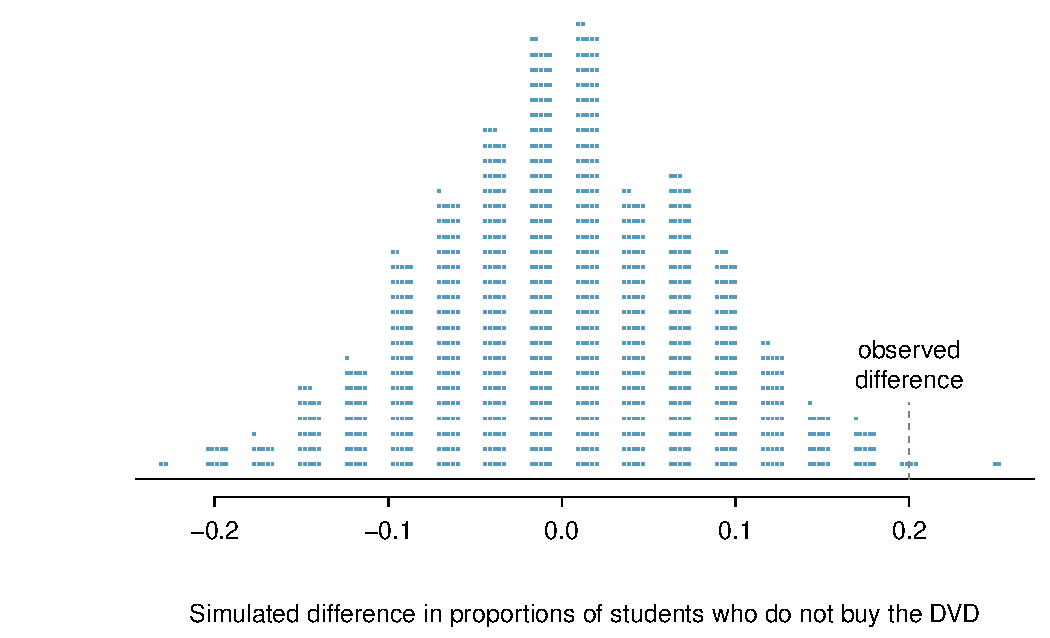
\includegraphics[width=0.93\textwidth]{05/figures/OpportunityCost/OpportunityCostDiffsDotPlot}
\caption{A stacked dot plot of 1,000 chance differences produced under the null hypothesis, $H_0$. Six of the 1,000 simulations had a difference of at least 20\%, which was the difference observed in the study.}
\label{OpportunityCostDiffsDotPlot}
\end{figure}

\begin{figure}[p]
\centering
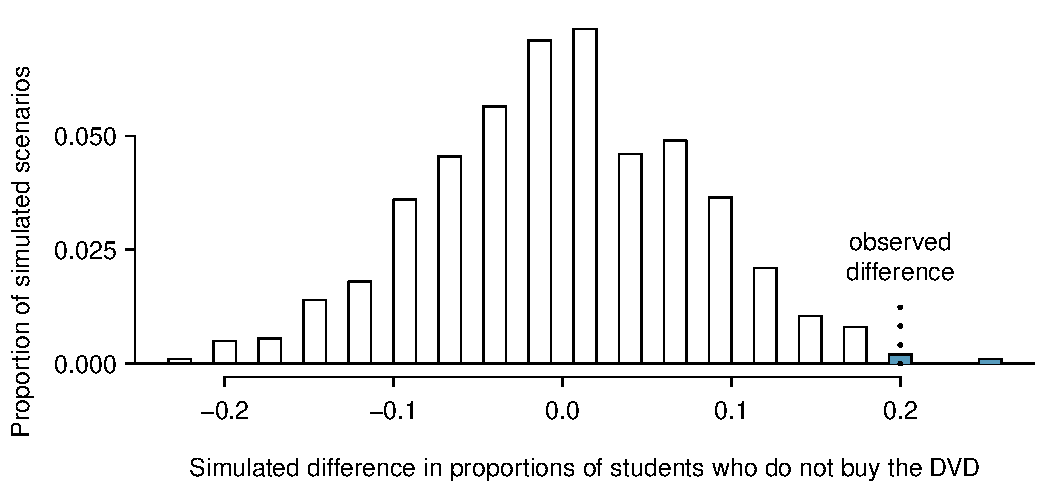
\includegraphics[width=0.93\textwidth]{05/figures/OpportunityCost/OpportunityCostDiffsRightTail}
\caption{A histogram of 1,000 chance differences produced under the null hypothesis, $H_0$. Histograms like this one are a more convenient representation of data or results when there are a large number of observations.}
\label{OpportunityCostDiffs}
\end{figure}

If there was no treatment effect, then we'd only observe a difference of at least +20\% about 0.6\% of the time, or about 1-in-150 times. That is really rare! Instead, we will conclude the data provide strong evidence there is a treatment effect: reminding students before a purchase that they could instead spend the money later on something else lowers the chance that they will continue with the purchase. Notice that we are able to make a causal statement for this study since the study is an experiment.

\textPE{\newpage}

%\begin{termBox}{\tBoxTitle{Become a savvy consumer}
%Apply what you just learned by signing a pledge saying that you will be a thoughtful consumer before you make a purchase. Visit \href{http://www.openintro.org/savvyconsumer}{openintro.org/savvyconsumer}.}
%\end{termBox}

%\Comment{Scrap box above? Or would it be fun? If keep, TODO(David): build a webpage for openintro.org/savvyconsumer.}



% conducted the study again with the same students. If the treatment had no influence on their decisions, each student would respond the same. We would still have 97 students would would buy the DVD and 53 students who would not. If we randomly split these students up into the treatment and control groups, we are simulating what might have happened if (1) we could repeat the study and (2) the null hypothesis was true, meaning the treatment has no effect.

%Table~\ref{} represents a new randomization of students into the treatment and control groups. In this simulation, we see that the 




%What if we could encourage more thoughtful spending by consumers by pointing out the obvious fact that they could spend money on different things? This was the 
%
%Capitalism is built on the premise that individuals make rational decision. What if we could 
%
%What if we told you there was a simple way to make people more thoughtful about how they spend their money?
%
%If shoppers are reminded that if they don't spend money today, they can spend it tomorrow, do you think that would have an influence on their shopping behavior?
%
%Consider the following scenario, which was given to 150 students:
%\begin{quote}
%Imagine that you have been saving some extra money on the side to make some purchases, and on your most recent visit to the video store you come across a special sale on a new video. This video is one with your favorite actor or actress, and your favorite type of movie (such as a comedy, drama, thriller, etc.). This particular video that you are considering is one you have been thinking about buying for a long time. It is available for a special sale price of \$14.99.
%\end{quote}


%%%%%
\section{Hypothesis testing}

%_________________
\section{Hypothesis testing}
\label{HypothesisTesting}

In the last two sections, we utilized a \term{hypothesis test}, which is a formal technique for evaluating two competing possibilities. In each scenario, we described a \term{null hypothesis}, which represented either a skeptical perspective or a perspective of no difference. We~also laid out an \term{alternative hypothesis}, which represented a new perspective such as the possibility that there has been a change or that there is a treatment effect in an experiment.

\begin{termBox}{\tBoxTitle{Null and alternative hypotheses}
The \term{null hypothesis ($H_0$)} often represents either a skeptical perspective or a claim to be tested. The \term{alternative hypothesis ($H_A$)} represents an alternative claim under consideration and is often represented by a range of possible values for the value of~interest.}
\end{termBox}

The hypothesis testing framework is a very general tool, and we often use it without a second thought. If a person makes a somewhat unbelievable claim, we are initially skeptical. However, if there is sufficient evidence that supports the claim, we set aside our skepticism. The hallmarks of hypothesis testing are also found in the US court system. 

\subsection{Hypothesis testing in the US court system}

\begin{example}{A US court considers two possible claims about a defendant: she is either innocent or guilty. If we set these claims up in a hypothesis framework, which would be the null hypothesis and which the alternative?}\label{hypTestCourtExample}
The jury considers whether the evidence is so convincing (strong) that there is no reasonable doubt regarding the person's guilt. That is, the skeptical perspective (null hypothesis) is that the person is innocent until evidence is presented that convinces the jury that the person is guilty (alternative hypothesis).
\end{example}

Jurors examine the evidence to see whether it convincingly shows a defendant is guilty. Notice that if a jury finds a defendant \emph{not guilty}, this does not necessarily mean the jury is confident in the person's innocence. They are simply not convinced of the alternative that the person is guilty.

This is also the case with hypothesis testing: \emph{even if we fail to reject the null hypothesis, we typically do not accept the null hypothesis as truth}. Failing to find strong evidence for the alternative hypothesis is not equivalent to providing evidence that the null hypothesis is true.


\subsection{p-value and statistical significance}

In Section~\ref{caseStudyGenderDiscrimination} we encountered a study from the 1970's that explored whether there was strong evidence that women were less likely to be promoted than men. The research question -- are females discriminated against in promotion decisions made by male managers? -- was framed in the context of hypotheses:
\begin{itemize}
\setlength{\itemsep}{0mm}
\item[$H_0$:] Gender has no effect on promotion decisions.
\item[$H_A$:] Women are discriminated against in promotion decisions.
\end{itemize}
The null hypothesis ($H_0$) was a perspective of no difference. The data, summarized on page~\pageref{discriminationResults}, provided a point estimate of a 29.2\% difference in recommended promotion rates between men and women. We determined that such a difference from chance alone would be rare: it would only happen about 2 in 100 times. When results like these are inconsistent with $H_0$, we reject $H_0$ in favor of $H_A$. Here, we concluded there was discrimination against women.

The 2-in-100 chance is what we call a \term{p-value}, which is a probability quantifying the strength of the evidence against the null hypothesis and in favor of the alternative. %Formally the p-value is a conditional probability, which is basically\footnote{Want to learn more probability? Check out~Appendix~\ref{probability}.}

\begin{termBox}{\tBoxTitle{p-value}
The \term{p-value}\index{hypothesis testing!p-value|textbf} is the probability of observing data at least as favorable to the alternative hypothesis as our current data set, if the null hypothesis were true. We~typically use a summary statistic of the data, such as a difference in proportions, to help compute the p-value and evaluate the~hypotheses. This summary value that is used to compute the p-value is often called the \term{test statistic}.}
\end{termBox}

\textA{\pagebreak}

\begin{example}{In the gender discrimination study, the difference in discrimination rates was our test statistic. What was the test statistic in the opportunity cost study covered in Section~\ref{caseStudyOpportunityCost}?}
The test statistic in the opportunity cost study was the difference in the proportion of students who decided against the DVD purchase in the treatment and control groups. In each of these examples, the \hiddenterm{point estimate} of the difference in proportions was used as the test statistic.
\end{example}

When the p-value is small, i.e. less than a previously set threshold, we say the results are \term{statistically significant}. This means the data provide such strong evidence against $H_0$ that we reject the null hypothesis in favor of the alternative hypothesis. The threshold, called the \term{significance level}\index{hypothesis testing!significance level}\index{significance level} and often represented by $\alpha$ (the Greek letter \emph{alpha}\label{alphadiscussion})\marginpar[\raggedright\vspace{-4mm}

$\alpha$\\\footnotesize significance\\level of a\\hypothesis test]{\raggedright\vspace{-4mm}

$\alpha$\\\footnotesize significance\\level of a\\hypothesis test}, is typically set to $\alpha = 0.05$, but can vary depending on the field or the application. Using a  significance level of $\alpha = 0.05$ in the discrimination study, we can say that the data provided statistically significant evidence against the null hypothesis.

\begin{termBox}{\tBoxTitle{Statistical significance}
We say that the data provide \term{statistically significant}\index{hypothesis testing!statistically significant|textbf} evidence against the null hypothesis if the p-value is less than some reference value, usually~$\alpha=0.05$.}
\end{termBox}

%\begin{termBox}{\tBoxTitle{Significance Level}
%If the null hypothesis is true, the significance level $\alpha$ defines the probability that we will make a Type~1 Error.}
%\end{termBox}

\begin{example}{In the opportunity cost study in Section~\ref{caseStudyOpportunityCost}, we analyzed an experiment where study participants were 20\% less likely to continue with a DVD purchase if they were reminded that the money, if not spent on the DVD, could be used for other purchases in the future. We determined that such a large difference would only occur about 1-in-150 times if the reminder actually had no influence on student decision-making. What is the p-value in this study? Was the result statistically significant?}
The p-value was 0.006 (about 1/150). Since the p-value is less than 0.05, the data provide statistically significant evidence that US college students were actually influenced by the reminder.
\end{example}

\begin{termBox}{\tBoxTitle{What's so special about 0.05?}
We often use a threshold of 0.05 to determine whether a result is statistically significant. But why 0.05? Maybe we should use a bigger number, or maybe a smaller number. If you're a little puzzled, that probably means you're reading with a critical eye -- good job! We've made a video to help clarify \emph{why 0.05}:
\begin{center}
\href{http://www.openintro.org/why05}{www.openintro.org/why05}
\end{center}
Sometimes it's also a good idea to deviate from the standard. We'll discuss when to choose a threshold different than 0.05 in Section~\ref{significanceLevel}.\vspace{0.5mm}}
\end{termBox}


\textA{\pagebreak}

\subsection{Decision errors}

\index{hypothesis testing!decision errors|(}

Hypothesis tests are not flawless. Just think of the court system: innocent people are sometimes wrongly convicted and the guilty sometimes walk free. Similarly, data can point to the wrong conclusion. However, what distinguishes statistical hypothesis tests from a court system is that our framework allows us to quantify and control how often the data lead us to the incorrect conclusion.

There are two competing hypotheses: the null and the alternative. In a hypothesis test, we make a statement about which one might be true, but we might choose incorrectly. There are four possible scenarios in a hypothesis test, which are summarized in Table~\ref{fourHTScenarios}.

\begin{table}[ht]
\centering
\begin{tabular}{l l c c c}
& & \multicolumn{2}{c}{\textbf{Test conclusion}} \\
  \cline{3-4}
\vspace{-3.7mm} \\
& & do not reject $H_0$ &  reject $H_0$ in favor of $H_A$ &
\ \hspace{7mm} \  \\
  \cline{2-4}
\vspace{-3.7mm} \\
& $H_0$ true & okay &  Type~1 Error \\
\raisebox{1.5ex}{\textbf{Truth}} & $H_A$ true & Type 2 Error & okay \\
  \cline{2-4}
\end{tabular}
\caption{Four different scenarios for hypothesis tests.}
\label{fourHTScenarios}
\end{table}

A \term{Type~1 Error} is rejecting the null hypothesis when $H_0$ is actually true. Since we rejected the null hypothesis in the gender discrimination and opportunity cost studies, it is possible that we made a Type~1 Error in one or both of those studies. A \term{Type~2 Error} is failing to reject the null hypothesis when the alternative is actually true.

\begin{example}{In a US court, the defendant is either innocent ($H_0$) or  guilty ($H_A$). What does a Type~1 Error represent in this context? What does a Type 2 Error represent? Table~\ref{fourHTScenarios} may be useful.}
If the court makes a Type~1 Error, this means the defendant is innocent ($H_0$ true) but wrongly convicted. A Type 2 Error means the court failed to reject $H_0$ (i.e. failed to convict the person) when she was in fact guilty ($H_A$ true).
\end{example}

\begin{exercise}
Consider the opportunity cost study where we concluded students were less likely to make a DVD purchase if they were reminded that money not spent now could be spent later. What would a Type~1 Error represent in this context?\footnote{Making a Type 1 Error in this context would mean that reminding students that money not spent now can be spent later does not affect their buying habits, despite the strong evidence (the data suggesting otherwise) found in the experiment. Notice that this does \emph{not} necessarily mean something was wrong with the data or that we made a computational mistake. Sometimes data simply point us to the wrong conclusion, which is why scientific studies are often repeated to check initial findings.}
\end{exercise}

\begin{example}{How could we reduce the Type~1 Error rate in US courts? What influence would this have on the Type 2 Error rate?}
To lower the Type~1 Error rate, we might raise our standard for conviction from ``beyond a reasonable doubt'' to ``beyond a conceivable doubt'' so fewer people would be wrongly convicted. However, this would also make it more difficult to convict the people who are actually guilty, so we would make more Type~2 Errors.
\end{example}

\begin{exercise} \label{howToReduceType2ErrorsInUSCourts}
How could we reduce the Type~2 Error rate in US courts? What influence would this have on the Type~1 Error rate?\footnote{To lower the Type~2 Error rate, we want to convict more guilty people. We could lower the standards for conviction from ``beyond a reasonable doubt'' to ``beyond a little doubt''. Lowering the bar for guilt will also result in more wrongful convictions, raising the Type~1 Error rate.}
\end{exercise}

\index{hypothesis testing!decision errors|)}

The example and guided practice above provide an important lesson: if we reduce how often we make one type of error, we generally make more of the other type.

%Hypothesis testing is built around rejecting or failing to reject the null hypothesis. That is, we do not reject $H_0$ unless the data provide strong evidence against it. But what precisely does \emph{strong evidence} mean? As a general rule of thumb, for those cases where the null hypothesis is actually true, we do not want to incorrectly reject $H_0$ more than 5\% of the time. This corresponds to our default significance level of $\alpha = 0.05$, which we use as a comparison with the p-value. In the next section, we discuss the appropriateness of different significance levels.


\subsection{Choosing a significance level}
\label{significanceLevel}

\index{hypothesis testing!significance level|(}
\index{significance level|(}

Choosing a significance level for a test is important in many contexts, and the traditional level is 0.05. However, it is sometimes helpful to adjust the significance level based on the application. We may select a level that is smaller or larger than 0.05 depending on the consequences of any conclusions reached from the test.

If making a Type~1 Error is dangerous or especially costly, we should choose a small significance level (e.g. 0.01 or 0.001). Under this scenario, we want to be very cautious about rejecting the null hypothesis, so we demand very strong evidence favoring the alternative $H_A$ before we would reject $H_0$.

If a Type 2 Error is relatively more dangerous or much more costly than a Type~1 Error, then we should choose a higher significance level (e.g. 0.10). Here we want to be cautious about failing to reject $H_0$ when the null is actually false.

\begin{tipBox}{\tipBoxTitle[]{Significance levels should reflect consequences of errors}
The significance level selected for a test should reflect the real-world consequences associated with making a Type~1 or Type 2 Error.}
\end{tipBox}


\subsection{Introducing two-sided hypotheses}
\label{IntroducingTwoSidedHypotheses}
%_________________
%\section[Case study: CPR and blood thinner (randomization)]{Case study: blood thinner and CPR\\(randomization)}

\index{hypothesis testing!two tails|(}

So far we have explored whether women were discriminated against and whether a simple trick could make students a little thriftier. In these two case studies, we've actually ignored some possibilities:
\begin{itemize}
\item What if \emph{men} are actually discriminated against?
\item What if the money trick actually makes students \emph{spend more}?
\end{itemize}
These possibilities weren't considered in our hypotheses or analyses. This may have seemed natural since the data pointed in the directions in which we framed the problems. However, there are two dangers if we ignore possibilities that disagree with our data or that conflict with our worldview:
\begin{enumerate}
\item Framing an alternative hypothesis simply to match the direction that the data point will generally inflate the Type 1 Error rate. After all the work we've done (and will continue to do) to rigorously control the error rates in hypothesis tests, careless construction of the alternative hypotheses can disrupt that hard work. We'll explore this topic further in Section~\ref{InflatingType1ErrorRate}.
\item If we only use alternative hypotheses that agree with our worldview, then we're going to be subjecting ourselves to \term{confirmation bias}, which means we are looking for data that supports our ideas. That's not very scientific, and we can do better!
\end{enumerate}
The previous hypotheses we've seen are called \term{one-sided hypothesis tests} because they only explored one direction of possibilities. Such hypotheses are appropriate when we are exclusively interested in the single direction, but usually we want to consider all possibilities. To~do~so, let's learn about \term{two-sided hypothesis tests} in the context of a new study that examines the impact of using blood thinners on patients who have undergone CPR.

\index{data!CPR and blood thinner|(}

Cardiopulmonary resuscitation (CPR) is a procedure used on individuals suffering a heart attack when other emergency resources are unavailable. This procedure is helpful in providing some blood circulation to keep a person alive, but CPR chest compressions can also cause internal injuries. Internal bleeding and other injuries that can result from CPR complicate additional treatment efforts. For instance, blood thinners may be used to help release a clot that is causing the heart attack once a patient arrives in the hospital. However, blood thinners negatively affect internal injuries.

Here we consider an experiment with patients who underwent CPR for a heart attack and were subsequently admitted to a hospital.\footnote{B$\ddot{\text{o}}$ttiger et al. ``Efficacy and safety of thrombolytic therapy after initially unsuccessful cardiopulmonary resuscitation: a prospective clinical trial.'' The Lancet, 2001.} Each patient was randomly assigned to either receive a blood thinner (treatment group) or not receive a blood thinner (control group). The outcome variable of interest was whether the patient survived for at least 24~hours.

% The way p_c and p_t are described make it sound like we are only considering the samples
\begin{example}{Form hypotheses for this study in plain and statistical language. Let $p_c$ represent the true survival rate of people who do not receive a blood thinner (corresponding to the control group) and $p_t$ represent the survival rate for people receiving a blood thinner (corresponding to the treatment group).} \label{hypothesesForCPRStudyInSmallSampleSection}
We want to understand whether blood thinners are helpful or harmful. We'll consider both of these possibilities using a two-sided hypothesis test.
\begin{itemize}
\item[$H_0$:] Blood thinners do not have an overall survival effect, i.e. the survival proportions are the same in each group. $p_t - p_c = 0$.
\item[$H_A$:] Blood thinners have an impact on survival, either positive or negative, but not zero. $p_t - p_c \neq 0$.
\end{itemize}
\end{example}

There were 50 patients in the experiment who did not receive a blood thinner and 40 patients who did. The study results are shown in Table~\ref{resultsForCPRStudyInSmallSampleSection}.

\begin{table}[ht]
\centering
\begin{tabular}{lccccc}
\hline
			&& Survived 	& Died 	&& Total \\
\hline
Control		&& 11		& 39		&& 50 \\
Treatment		&& 14		& 26		&& 40 \\
\hline
Total			&& 25		& 65		&& 90 \\
\hline
\end{tabular}
\caption{Results for the CPR study. Patients in the treatment group were given a blood thinner, and patients in the control group were not.}
\label{resultsForCPRStudyInSmallSampleSection}
\end{table}

\begin{exercise}
What is the observed survival rate in the control group? And in the treatment group? Also, provide a point estimate of the difference in survival proportions of the two groups: $\hat{p}_t - \hat{p}_c$.~\footnote{Observed control survival rate: $p_c = \frac{11}{50} = 0.22$. Treatment survival rate: $p_t = \frac{14}{40} = 0.35$. Observed difference: $\hat{p}_t - \hat{p}_c = 0.35 - 0.22 = 0.13$.}
\end{exercise}

According to the point estimate, for patients who have undergone CPR outside of the hospital, an additional 13\% of these patients survive when they are treated with blood thinners. However, we wonder if this difference could be easily explainable by chance.

As we did in our past two studies this chapter, we will simulate what type of differences we might see from chance alone under the null hypothesis. By randomly assigning ``simulated treatment'' and ``simulated control'' stickers to the patients' files, we get a new grouping. If we repeat this simulation 10,000 times, we can build a \term{null distribution} of the differences shown in Figure~\ref{CPR_study_right_tail}.

\begin{figure}[ht]
\centering
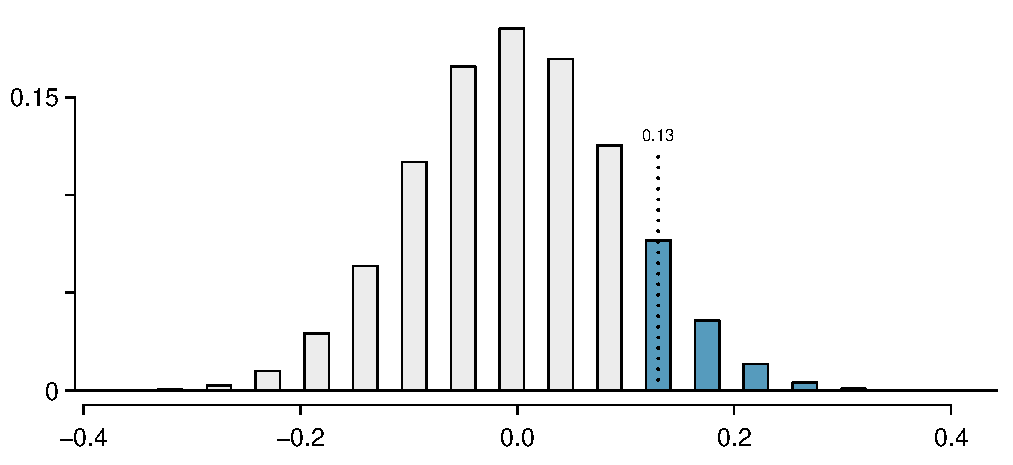
\includegraphics[width=0.8\textwidth]{05/figures/CPR_study/CPR_study_right_tail}
\caption{Null distribution of the point estimate, $\hat{p}_t - \hat{p}_c$. The shaded right tail shows observations that are at least as large as the observed difference,~0.13.}
\label{CPR_study_right_tail}
\end{figure}

The right tail area is about 0.13. (Note: it is only a coincidence that we also have $\hat{p}_t - \hat{p}_c=0.13$.) However, contrary to how we calculated the p-value in previous studies, the p-value of this test is not~0.13!

The p-value is defined as the chance we observe a result at least as favorable to the alternative hypothesis as the result (i.e.~the difference) we observe. In this case, any differences less than or equal to -0.13 would also provide equally strong evidence favoring the alternative hypothesis as a difference of 0.13. A difference of -0.13 would correspond to 13\% higher survival rate in the control group than the treatment group. In Figure~\ref{CPR_study_p_value} we've also shaded these differences in the left tail of the distribution. These two shaded tails provide a visual representation of the p-value for a two-sided test.

%There is something different in this study than in the past studies: in this study, we are particularly interested in whether blood thinners increase \emph{or} decrease the risk of death in patients who undergo CPR before arriving at the hospital.\footnote{Realistically, we probably are interested in either direction in the past studies as well, and so we should have used the approach we now discuss in this section. However, for simplicity and the sake of not introducing too many concepts at once, we skipped over these details in earlier sections.} For example, there are chance differences of $\hat{p}_t - \hat{p}_c = -0.14$, that would have been stronger evidence against the null hypothesis as our observed difference of +0.13. Likewise, anything less than or equal -0.13 would provide as much evidence against the null hypothesis as +0.13, and for this reason, we must count both tails towards the p-value, as shown in Figure~\ref{CPR_study_p_value}.

\begin{figure}[ht]
\centering
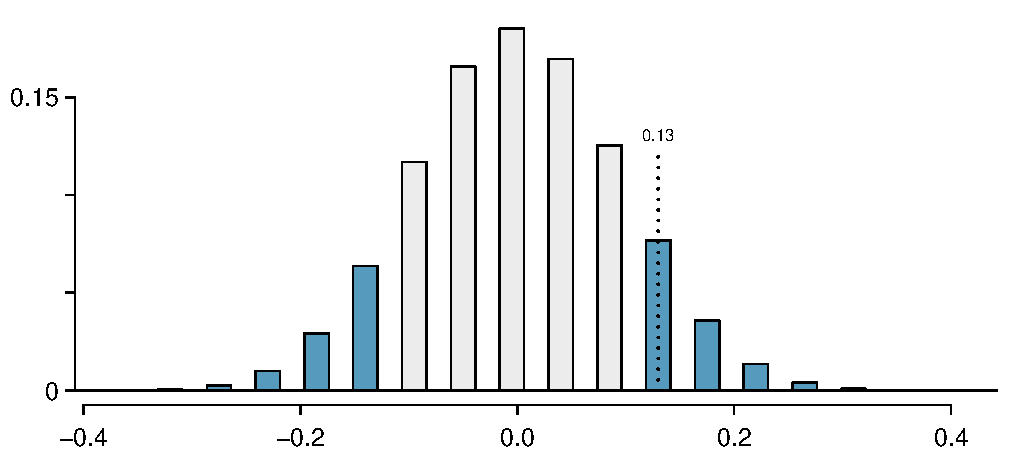
\includegraphics[width=0.7\textwidth]{05/figures/CPR_study/CPR_study_p_value}
\caption{Null distribution of the point estimate, $\hat{p}_t - \hat{p}_c$. All values that are at least as extreme as +0.13 but in either direction away from~0 are~shaded.}
\label{CPR_study_p_value}
\end{figure}

For a two-sided test, take the single tail (in this case, 0.13) and double it to get the p-value: 0.26. Since this p-value is larger than 0.05, we do not reject the null hypothesis. That is, we do not find statistically significant evidence that the blood thinner has any influence on survival of patients who undergo CPR prior to arriving at the hospital. %Once again, we can discuss the causal conclusion since this is an experiment.

\index{data!CPR and blood thinner|)}

\begin{termBox}{\tBoxTitle{Default to a two-sided test}
We want to be rigorous and keep an open mind when we analyze data and evidence. Use a one-sided hypothesis test only if you truly have interest in only one direction.}
\end{termBox}

\begin{termBox}{\tBoxTitle{Computing a p-value for a two-sided test}
First compute the p-value for one tail of the distribution, then double that value to get the two-sided p-value. That's it!}
\end{termBox}


\subsection{Controlling the Type~1 Error~rate}
\label{InflatingType1ErrorRate}

It is never okay to change two-sided tests to one-sided tests after observing the data. We explore the consequences of ignoring this advice in the next example.

\begin{example}{Using $\alpha=0.05$, we show that freely switching from two-sided tests to one-sided tests will lead us to make twice as many Type~1 Errors as intended.} \label{swappingHypAfterDataDoublesType1ErrorRate}
Suppose we are interested in finding any difference from 0. We've created a smooth-looking \term{null distribution} representing differences due to chance in Figure~\ref{type1ErrorDoublingExampleFigure}.

\begin{figure}[h]
\centering
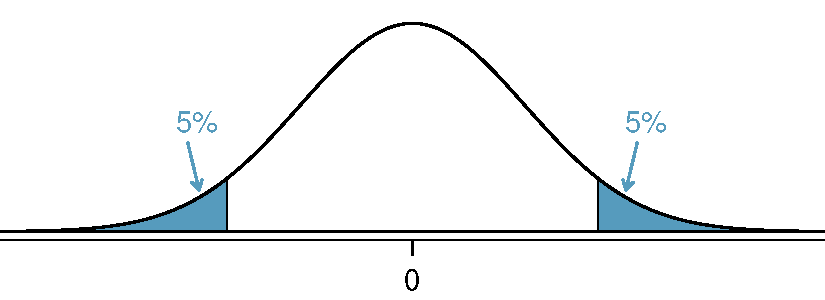
\includegraphics[width=0.7\textwidth]{05/figures/type1ErrorDoublingExampleFigure/type1ErrorDoublingExampleFigure}
\caption{The shaded regions represent areas where we would reject $H_0$ under the bad practices considered in Example~\ref{swappingHypAfterDataDoublesType1ErrorRate} when $\alpha = 0.05$.}
\label{type1ErrorDoublingExampleFigure}
\end{figure}

Suppose the sample difference was larger than 0. Then if we can flip to a one-sided test, we would use $H_A$: difference $> 0$. Now if we obtain any observation in the upper 5\% of the distribution, we would reject $H_0$ since the p-value would just be a the single tail. Thus, if the null hypothesis is true, we incorrectly reject the null hypothesis about 5\% of the time when the sample mean is above the null value, as shown in Figure~\ref{type1ErrorDoublingExampleFigure}.

Suppose the sample difference was smaller than 0. Then if we change to a one-sided test, we would use $H_A$: difference $< 0$. If the observed difference falls in the lower 5\% of the figure, we would reject $H_0$. That is, if the null hypothesis is true, then we would observe this situation about 5\% of the time.

By examining these two scenarios, we can determine that we will make a Type~1 Error $5\%+5\%=10\%$ of the time if we are allowed to swap to the ``best'' one-sided test for the data. This is twice the error rate we prescribed with our significance level: $\alpha=0.05$ (!).
\end{example}

\begin{caution}{Hypothesis tests should be set up \emph{before} seeing the data}
{After observing data, it is tempting to turn a two-sided test into a one-sided test. Avoid this temptation. Hypotheses should be set up \emph{before} observing the data.}
\end{caution}

%\Comment{Should we scrap this subsection and example and just leave the caution box? Downside: weakens item 1 near the start of Section~\ref{IntroducingTwoSidedHypotheses}.}

\index{hypothesis testing!two tails|)}


\subsection{How to use a hypothesis test}

\noindent\textbf{Frame the research question in terms of hypotheses.} Hypothesis tests are appropriate for research questions that can be summarized in two competing hypotheses. The null hypothesis ($H_0$) usually represents a skeptical perspective or a perspective of no difference. The alternative hypothesis ($H_A$) usually represents a new view or a difference. \\

\noindent\textbf{Collect data with an observational study or experiment.} If a research question can be formed into two hypotheses, we can collect data to run a hypothesis test. If the research question focuses on associations between variables but does not concern causation, we would run an observational study. If the research question seeks a causal connection between two or more variables, then an experiment should be used. \\

\noindent\textbf{Analyze the data.} Choose an analysis technique appropriate for the data and identify the p-value. So far, we've only seen one analysis technique: randomization. Throughout the rest of this textbook, we'll encounter several new methods suitable for many other contexts. \\

\noindent\textbf{Form a conclusion.} Using the p-value from the analysis, determine whether the data provide statistically significant evidence against the null hypothesis. Also, be sure to write the conclusion in plain language so casual readers can understand the results.

\textPE{\newpage}


%%%%%
\section{Confidence intervals}

% new content based on bootstrapping
% can borrow language from old files on CIs (not included here since most wouldn't be used)

%%%%%
\section{Simulation case studies}

%_________________
\section{Simulation case studies}
\label{SimulationCaseStudies}

Randomization is a statistical technique suitable for evaluating whether a difference in sample proportions is due to chance. In this section, we explore the situation where we focus on a single proportion, and we introduce a new simulation method.

\subsection{Medical consultant}

\index{data!medical consultant|(}
People providing an organ for donation sometimes seek the help of a special medical consultant. These consultants assist the patient in all aspects of the surgery, with the goal of reducing the possibility of complications during the medical procedure and recovery. Patients might choose a consultant based in part on the historical complication rate of the consultant's clients.

One consultant tried to attract patients by noting the average complication rate for liver donor surgeries in the US is about 10\%, but her clients have had only 3 complications in the 62 liver donor surgeries she has facilitated. She claims this is strong evidence that her work meaningfully contributes to reducing complications (and therefore she should be~hired!).

\begin{example}{We will let $p$ represent the true complication rate for liver donors working with this consultant. Estimate $p$ using the data, and label this value $\hat{p}$.}
The sample proportion for the complication rate is 3~complications divided by the 62~surgeries the consultant has worked on: $\hat{p} = 3/62 = 0.048$.
\end{example}

\begin{example}{Is it possible to assess the consultant's claim using the data?}
No. The claim is that there is a causal connection, but the data are observational. For example, maybe patients who can afford a medical consultant can afford better medical care, which can also lead to a lower complication rate.

While it is not possible to assess the causal claim, it is still possible to test for an association using these data. For this question we ask, could the low complication rate of $\hat{p} = 0.048$ be due to chance?
\end{example}

\begin{example}{We're going to conduct a hypothesis test for this setting. Should the test be one-sided or two-sided?}
The setting has been framed in the context of the consultant being helpful, but what if the consultant actually performed worse than the average? Would we care? More than ever! Since we care about a finding in either direction, we should run a two-sided~test.
\end{example}

\begin{exercise}\label{hypForAssessingConsultantWorkInLiverTransplants}
Write out hypotheses in both plain and statistical language to test for the association between the consultant's work and the true complication rate, $p$, for this consultant's clients.\footnote{$H_0$: There is no association between the consultant's contributions and the clients' complication rate. That~is, the complication rate for the consultant's clients is equal to the US average of 10\%. In statistical language, $p=0.10$. $H_A$: Patients who work with the consultant have a complication rate different than~10\%, i.e.~$p \neq 0.10$.}
\end{exercise}

\begin{termBox}{\tBoxTitle{Parameter for a hypothesis test}
A \term{parameter} for a hypothesis test is the ``true'' value of interest. We typically estimate the parameter using a point estimate\index{point estimate} from a sample of data. \vspace{3mm}

For example, we estimate the probability $p$ of a complication for a client of the medical consultant by examining the past complications rates of her clients:\vspace{-2mm}
\begin{align*}
\hat{p} = 3 / 62 = 0.048\qquad\text{is used to estimate}\qquad p
\end{align*}}
\end{termBox}

%\begin{termBox}{\tBoxTitle{Point estimates vs parameter}\index{point estimate}\index{parameter}
%Point estimates are calculated based on a sample. For example, the \emph{observed} complication rate for the medical consultant's patients is $\hat{p} = 0.048$. This point estimate is our best guess at the probability $p$ a randomly selected client of hers has a complication. This probability is the parameter and its precise value is never known. However, we can estimate it using the point estimate $\hat{p}$.}
%\end{termBox}

\begin{termBox}{\tBoxTitle{Null value of a hypothesis test}
The \term{null value} is the reference value for the parameter in $H_0$, and it is sometimes represented with the parameter's label with a~subscript 0, e.g.~$p_0$ (just like $H_0$).}
\end{termBox}

In the medical consultant case study, the parameter is $p$ and the null value is $p_0 = 0.10$. We will use the p-value to quantify the possibility of a sample proportion ($\hat{p}$) this far from the null value. The p-value is computed based on the null distribution, which is the distribution of the test statistic if the null hypothesis were true. Just like we did using randomization for a difference in proportions, here we can simulate 62 new patients to see what result might happen if the complication rate was 0.10.

Each client can be simulated using a deck of cards. Take one red card, nine black cards, and mix them up. If the cards are well-shuffled, drawing the top card is one way of simulating the chance a patient has a complication if the true rate is 0.10: if the card is red, we say the patient had a complication, and if it is black then we say they did not have a complication. If we repeat this process 62 times and compute the proportion of simulated patients with complications, $\hat{p}_{sim}$, then this simulated proportion is exactly a draw from the null distribution.

\begin{exercise}
In a simulation of 62 patients, about how many would we expect to have had a complication?\footnote{About 10\% of the patients (6.2 on average) in the simulation will have a complication, though we will see a little variation from one simulation to the next.}
\end{exercise}

We conducted such a simulation. There were 5 simulated cases with a complication and 57 simulated cases without a complication: $\hat{p}_{sim} = 5/62 = 0.081$.

One simulation isn't enough to get a sense of the null distribution, so we repeated the simulation 10,000 times using a~computer. Figure~\ref{MedConsNullSim} shows the null distribution from these 10,000 simulations. The simulated proportions that are less than or equal to $\hat{p}=0.048$ are shaded. There were 1222 simulated sample proportions with $\hat{p}_{sim} \leq 0.048$, which represents a fraction 0.1222 of our simulations:
\begin{align*}
\text{left tail }
	= \frac{\text{Number of observed simulations with }\hat{p}_{sim}\leq\text{ 0.048}}{10000}
	= \frac{1222}{10000} = 0.1222
\end{align*}
However, this is not our p-value! Remember that we are conducting a two-sided test, so we should double the one-tail area to get the p-value:\footnote{This doubling approach is preferred even when the distribution isn't symmetric, as in this case.}
\begin{align*}
\text{p-value} = 2 \times \text{left tail} = 2 \times 0.1222 = 0.2444
\end{align*}

\begin{figure}[ht]
\centering
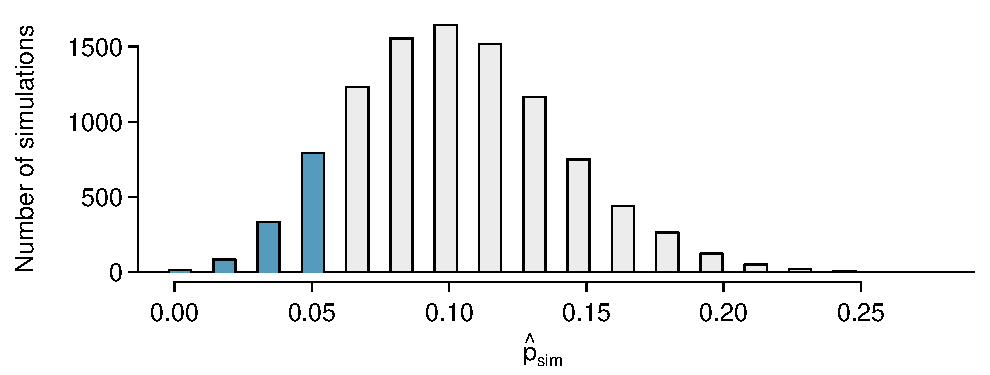
\includegraphics[width=0.83\textwidth]{05/figures/MedicalConsultant/MedConsNullSim}
\caption{The null distribution for $\hat{p}$, created from 10,000 simulated studies. The left tail contains 12.22\% of the simulations. We double this value to get the p-value.}
\label{MedConsNullSim}
\end{figure}

\begin{exercise} \label{plainLanguageExplanationOfHTConclusionForLiverDonorSurgicalConsultant}
Because the p-value is 0.2444, which is larger than the significance level 0.05, we do not reject the null hypothesis. Explain what this means in the context of the problem using plain language.\footnote{The data do not provide strong evidence that the consultant's work is associated with a lower or higher rate of surgery complications than the general rate of 10\%.}
\end{exercise}

\begin{example}{Does the conclusion in Guided Practice~\ref{plainLanguageExplanationOfHTConclusionForLiverDonorSurgicalConsultant} imply there is no real association between the surgical consultant's work and the risk of complications? Explain.}
No. It might be that the consultant's work is associated with a lower or higher risk of complications. However, the data did not provide enough information to reject the null hypothesis. %However, we currently don't have enough data to say whether the corresponding complication rate is any different than 0.10.
\index{data!medical consultant|)}
\end{example}


%_________________
\subsection{Tappers and listeners}

Here's a game you can try with your friends or family: pick a simple, well-known song, tap that tune on your desk, and see if the other person can guess the song. In this simple game, you are the tapper, and the other person is the listener.

A Stanford University graduate student named Elizabeth Newton conducted an experiment using the tapper-listener game.\footnote{This case study is described in \emph{\href{http://www.openintro.org/redirect.php?go=made-to-stick&redirect=simulation_textbook_pdf_preliminary}{Made to Stick}} by Chip and Dan Heath. Little known fact: the teaching principles behind many OpenIntro resources are based on \emph{Made to Stick}.} In her study, she recruited 120 tappers and 120 listeners into the study. About 50\% of the tappers expected that the listener would be able to guess the song. Newton wondered, is 50\% a reasonable expectation?

Newton's research question can be framed into two hypotheses:
\begin{itemize}
\setlength{\itemsep}{0mm}
\item[$H_0$:] The tappers are correct, and generally 50\% of the time listeners are able to guess the tune. $p = 0.50$
\item[$H_A$:] The tappers are incorrect, and either more than or less than 50\% of listeners will be able to guess the tune. $p \neq 0.50$
\end{itemize}

In Newton's study, only 3 out of 120 listeners ($\hat{p} = 0.025$) were able to guess the tune! From the perspective of the null hypothesis, we might wonder, how likely is it that we would get this result from chance alone? That is, what's the chance we would happen to see such a small fraction if $H_0$ were true and the true correct-guess rate is 0.50?

We will again use a simulation. To simulate 120 games under the null hypothesis where $p = 0.50$, we could flip a coin 120 times. Each time the coin came up heads, this could represent the listener guessing correctly, and tails would represent the listener guessing incorrectly. For example, we can simulate 5 tapper-listener pairs by flipping a coin 5~times:
\begin{center}
\begin{tabular}{ccc ccc ccc c}
H & H & T & H & T \\
Correct & Correct & Wrong & Correct & Wrong \\
\end{tabular}
\end{center}
After flipping the coin 120 times, we got 56 heads for $\hat{p}_{sim} = 0.467$. As we did with the randomization technique, seeing what would happen with one simulation isn't enough. In order to evaluate whether our originally observed proportion of 0.025 is unusual or not, we should generate more simulations. Here we've repeated this simulation ten times:
\begin{align*}
0.558 \quad 0.517 \quad 0.467 \quad 0.458 \quad
0.525 \quad 0.425 \quad 0.458 \quad 0.492 \quad
0.550 \quad 0.483
\end{align*} % round(rbinom(10, 120, 0.5) / 120, 3)
As before, we'll run a total of 10,000 simulations using a computer. Figure~\ref{TappersAndListenersNullDistribution} shows the results of these simulations. Even in these 10,000 simulations, we don't see any results close to 0.025.

\begin{figure}[ht]
\centering
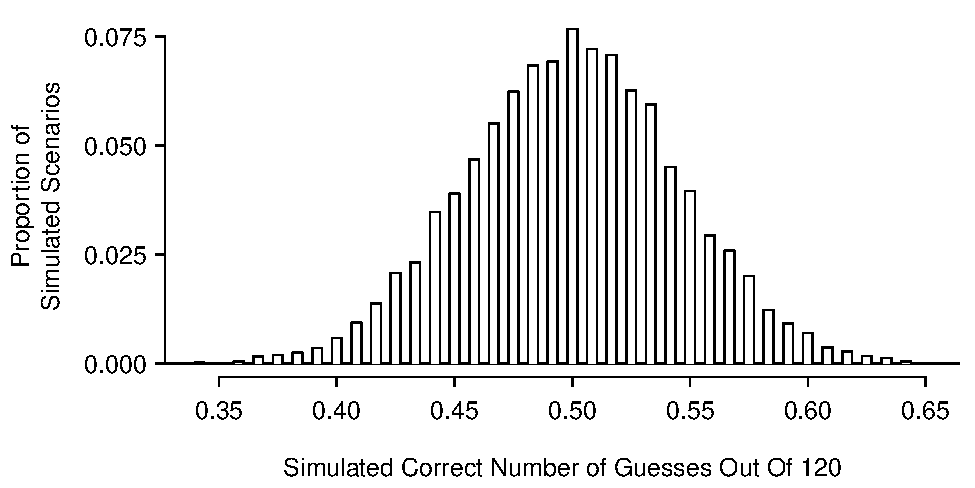
\includegraphics[width=0.8\textwidth]{05/figures/TappersAndListeners/TappersAndListenersNullDistribution}
\caption{Results from 10,000 simulations of the tapper-listener study where guesses are correct half of the time.}
\label{TappersAndListenersNullDistribution}
\end{figure}

\begin{exercise}
What is the p-value for the hypothesis test?\footnote{The p-value is the chance of seeing the data summary or something more in favor of the alternative hypothesis. Since we didn't observe anything even close to just 3 correct, the p-value will be small, around 1-in-10,000 or smaller.}
\end{exercise}

\begin{exercise}
Do the data provide statistically significant evidence against the null hypothesis? State an appropriate conclusion in the context of the research question.\footnote{The p-value is less than 0.05, so we reject the null hypothesis. There is statistically significant evidence, and the data provide strong evidence that the chance a listener will guess the correct tune is less than 50\%.}
\end{exercise}

% CONSIDER: adding a note about statistical software here and/or benefits of normal model to be introduced.

\textPE{\newpage}
